\documentclass[a4paper,10pt]{article}
\usepackage[english]{babel}
\usepackage{amsthm, amsmath, amssymb, amsfonts, nicefrac, mathpazo} 
\usepackage{graphicx}
\usepackage{listings, color}
\usepackage{fancyhdr, fullpage}
\usepackage{caption, float}
\usepackage{subcaption}
\usepackage{csquotes}

\definecolor{codegreen}{rgb}{0,0.6,0}
\definecolor{codegray}{rgb}{0.5,0.5,0.5}
\definecolor{codepurple}{rgb}{0.58,0,0.82}
\definecolor{backcolour}{rgb}{0.95,0.95,0.92}
\definecolor{codeblue}{rgb}{0,0,1}
 
\lstdefinestyle{mystyle}{
    backgroundcolor=\color{backcolour},   
    commentstyle=\color{codegreen},
    keywordstyle=\color{codeblue},
    numberstyle=\tiny\color{codegray},
    stringstyle=\color{codepurple},
    basicstyle=\footnotesize,
    breakatwhitespace=false,         
    breaklines=true,                 
    captionpos=b,                    
    keepspaces=true,                 
    numbers=left,                    
    numbersep=5pt,                  
    showspaces=false,                
    showstringspaces=false,
    showtabs=false,                  
    tabsize=2
}
 
\lstset{style=mystyle}

%Easier to call Naturals, Integers and so on.
\newcommand{\N}{\mathbb{N}}
\newcommand{\Z}{\mathbb{Z}}
\newcommand{\Q}{\mathbb{Q}}
\newcommand{\C}{\mathbb{C}}
\newcommand{\ind}{1\hspace{-2.1mm}{1}} %Indicator Function
\newcommand{\I}{\mathtt{i}}
\newcommand{\EE}{\mathbb{E}}
\newcommand{\RR}{\mathbb{R}}
\newcommand{\PP}{\mathbb{P}}
\newcommand{\D}{\mathrm{d}}
\newcommand{\Xe}{X^{\varepsilon}}
\newcommand{\E}{\mathrm{e}}
\newcommand{\Tr}{\mathrm{Tr}}
\newcommand{\HH}{\mathrm{H}}
\newcommand{\sgn}{\mathrm{sgn}}
\newcommand{\atanh}{\mathrm{arctanh}}
\def\equalDistrib{\,{\buildrel \Delta \over =}\,}

\setlength{\headheight}{13.6pt}
%%%%%%%%%%%%%%%%%%%%%%%%%%%%%%%%%%%%%%%%%%%%%%%%%%%%%%%%%%%%
\title{M4N9: Project 0}
\author{Yadu Bhageria}
\date{February 2016}

\pagestyle{fancy}
\fancyhf{}
\rhead{CID:00733164}
\lhead{Yadu Bhageria}
\rfoot{Page \thepage}

\begin{document}

\begin{titlepage}
    \begin{center}
    
        Coursework report presented for\\
        M4N9
        
        \vfill
        
        {\Huge Computational Linear Algebra\\ Project 0}
        
        
        \vspace{0.5cm}
        %subtitle?
        
        \vspace{1.5cm}
        
        {\Large Yadu \emph{Bhageria}}
        
        \vfill
        
        Mathematics Department\\
        Imperial College London\\
        United Kingdom\\
        \today
        
    \end{center}
\end{titlepage}

%%%%%%%%%%%%%%%%%%%%%%%%%%%%%%%%%%%%%%%%%%%%%%%%%%%%%%%%%%%%
%%%%%%%%%%%%%%%%%%%%%%%%%%%%%%%%%%%%%%%%%%%%%%%%%%%%%%%%%%%%
\textbf{ }
\section{Part a}

The modified modified Gram-Schmidt algorithm takes into account the weighted norm rather than the standard norm. This changes two steps of the algorithm. 

Firstly we change $$ r_{ii} = \|v_i\|_2 \quad \text{ to } \quad r_{ii} = \|v_i\|_W = \langle v_i, v_i \rangle_W^{\frac{1}{2}} $$

And secondly we change $$ r_{ij} = q_i^{\star}v_j \quad \text{ to } \quad r_{ij} = \langle q_i, v_j \rangle_W $$

Note that the discrete inner product is proportional to an approximation of the continuous one. Since I have to normalise all the vectors later anyways I can avoid multiplying the inner products by $\Delta x $. Thus I take $$ q_i^\star v_j = \Sigma_{k=1}^m q_{ik} v_{kj} w_k \quad \text{ and } \quad \|v_i\|_W = (\Sigma_{k=1}^m v_{ik} v_{ik} w_k)^{\frac{1}{2}} $$
where $ w_i = (1-x_i^2)^{\frac{1}{2}} $\\

Also, in order to normalise the polynomials I choose the last point of my x vector, $x_m$ which is just below the value of 1, i.e. $x_m < 1$ . This almost guarantees that none of my polynomials will take a value of 0 at this point and thus I can normalise with confidence. 

A plot for the resulting polynomials for n = 8 and m = 128 is given below

\begin{center}
	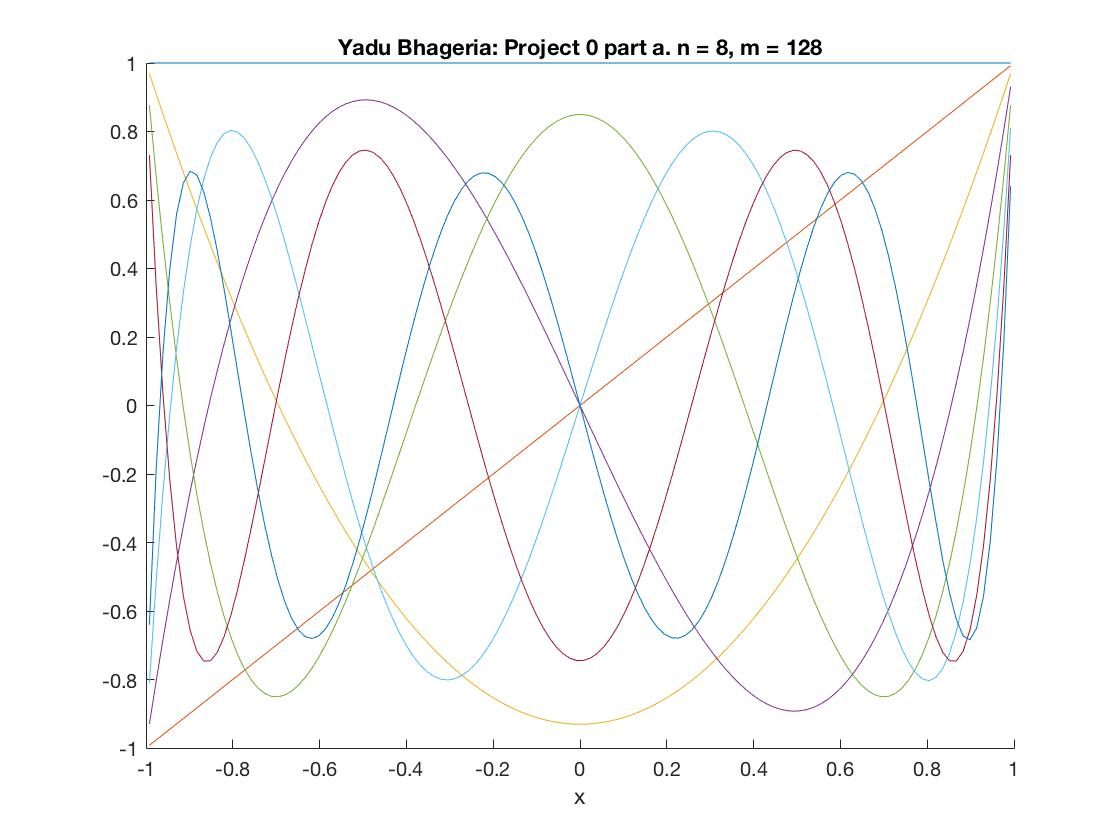
\includegraphics[width=0.8\textwidth]{fig_a.jpg}
\end{center}

%%%%%%%%%%%%%%%%%%%%%%%%%%%%%%%%%%%%%%%%%%%%%%%%%%%%%%%%%%%%
%%%%%%%%%%%%%%%%%%%%%%%%%%%%%%%%%%%%%%%%%%%%%%%%%%%%%%%%%%%%
\newpage
\section{Part b}

Choosing instead the points $x_i = \cos(\pi(2i − 1)/(2m)$ with $i=1,\dots,m$ can be thought of by considering the substitution $x = \cos(\theta) $. Which gives 

\begin{equation*}
	\begin{split}
		\int_{-1}^1 T_n(x) T_m(x) (1 - x^2)^(\frac{1}{2}) dx & = \int_{-1}^1 T_n( \cos( \theta)) T_m( \cos( \theta)) \frac{1}{\sqrt{1-\cos(\theta)^2}} dx \\
		& = \int_{\pi}^0 T_n( \cos( \theta)) T_m( \cos( \theta)) \frac{1}{\sin(\theta)} -\sin(\theta) d\theta \\
		& = \int_{0}^\pi T_n( \cos( \theta)) T_m( \cos( \theta)) d\theta \\
	\end{split}
\end{equation*}

 This can be thought of as points spaced evenly for $\theta \in [0,\pi)$ and so we take $x = cos(\theta)$ which over this interval giving $x_i = \cos(\pi(2i − 1)/(2m)$. The inner product can now we taken as $$ q_i^\star v_j = \Sigma_{k=1}^m q_{ik} v_{kj} \quad \text{ and } \quad \|v_i\|_W = (\Sigma_{k=1}^m v_{ik} v_{ik})^{\frac{1}{2}} $$ as this holds up to proportionality.

A plot for the resulting polynomials for n = 8 and m = 128 is given below

\begin{center}
	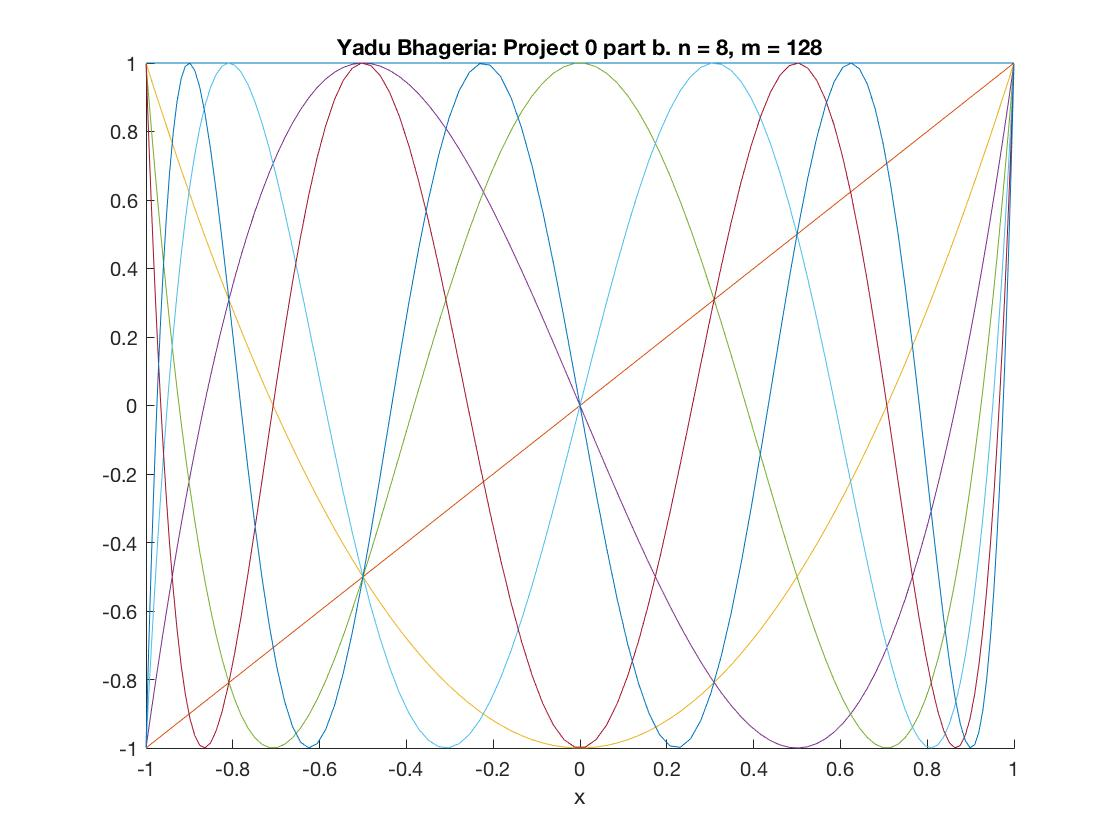
\includegraphics[width=0.8\textwidth]{fig_b.jpg}
\end{center}

%%%%%%%%%%%%%%%%%%%%%%%%%%%%%%%%%%%%%%%%%%%%%%%%%%%%%%%%%%%%
%%%%%%%%%%%%%%%%%%%%%%%%%%%%%%%%%%%%%%%%%%%%%%%%%%%%%%%%%%%%
\section{Part c}

In this section I take the error for the standard modified Gram-Schmidt as give below

$$
	E_s = \sqrt{ \Delta \theta \quad \Sigma_{i=1}^m ( T_n(x) - T^\sim_n(x))^2}
$$

I get the following the results for errors for the two methods. mmgs is the modified modified Gram-Schmidt whereas smgs is the standard modified Gram-Schmidt which is used with the $x=\cos(\theta)$ substitution.

\begin{verbatim}

Table_mmgs = 

             M128        M256        M512       M1024  
           ________    ________    ________    ________

    T_2    0.075029    0.052655     0.03709    0.026176
    T_4     0.17938     0.12186    0.084408    0.059056
    T_8     0.47872     0.28697     0.18595     0.12562


Table_smgs = 

              M128          M256          M512         M1024   
           __________    __________    __________    __________

    T_2    6.0052e-16    1.6768e-16    5.9824e-16    1.7849e-16
    T_4    1.6946e-15    1.0561e-15    1.2704e-15    1.4189e-15
    T_8    3.6979e-14    2.2235e-14    2.4762e-14    3.0564e-14
\end{verbatim}

It is clear that the second approach provides the better approximation. This can be seen by inspecting the errors and plots. 

\begin{center}
	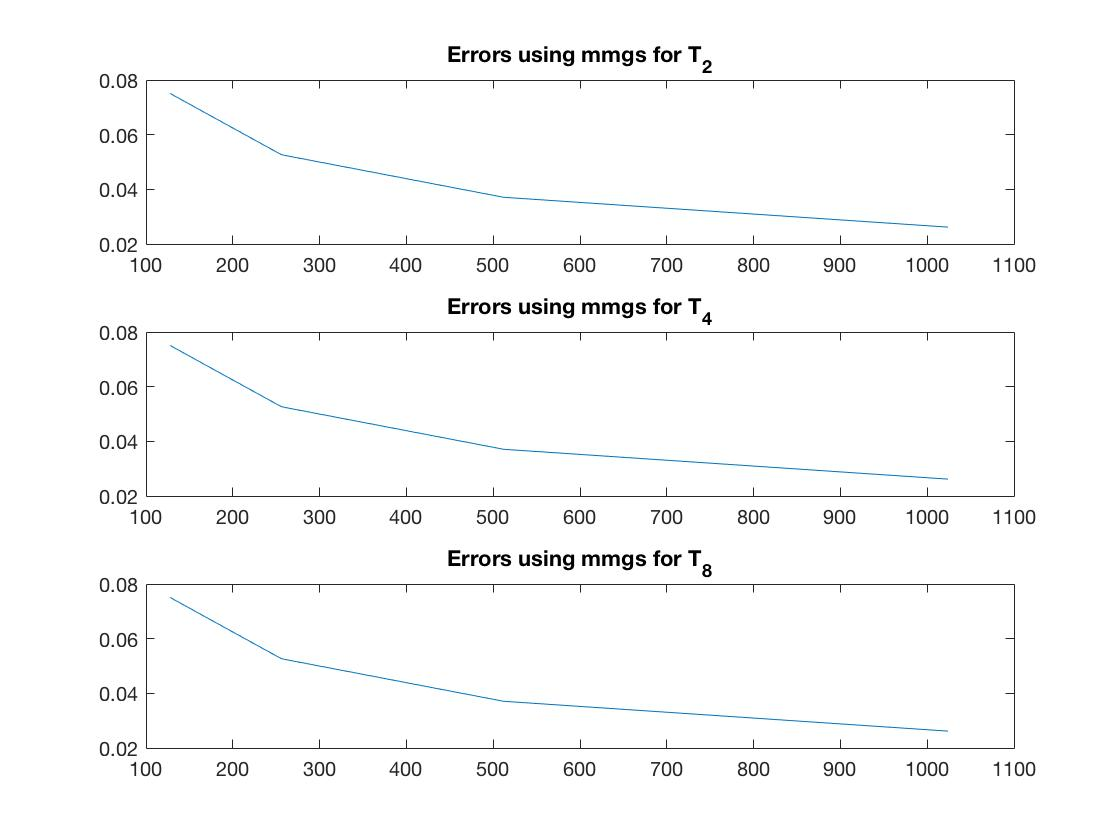
\includegraphics[width=0.49\textwidth]{fig_e_mmgs.jpg}
	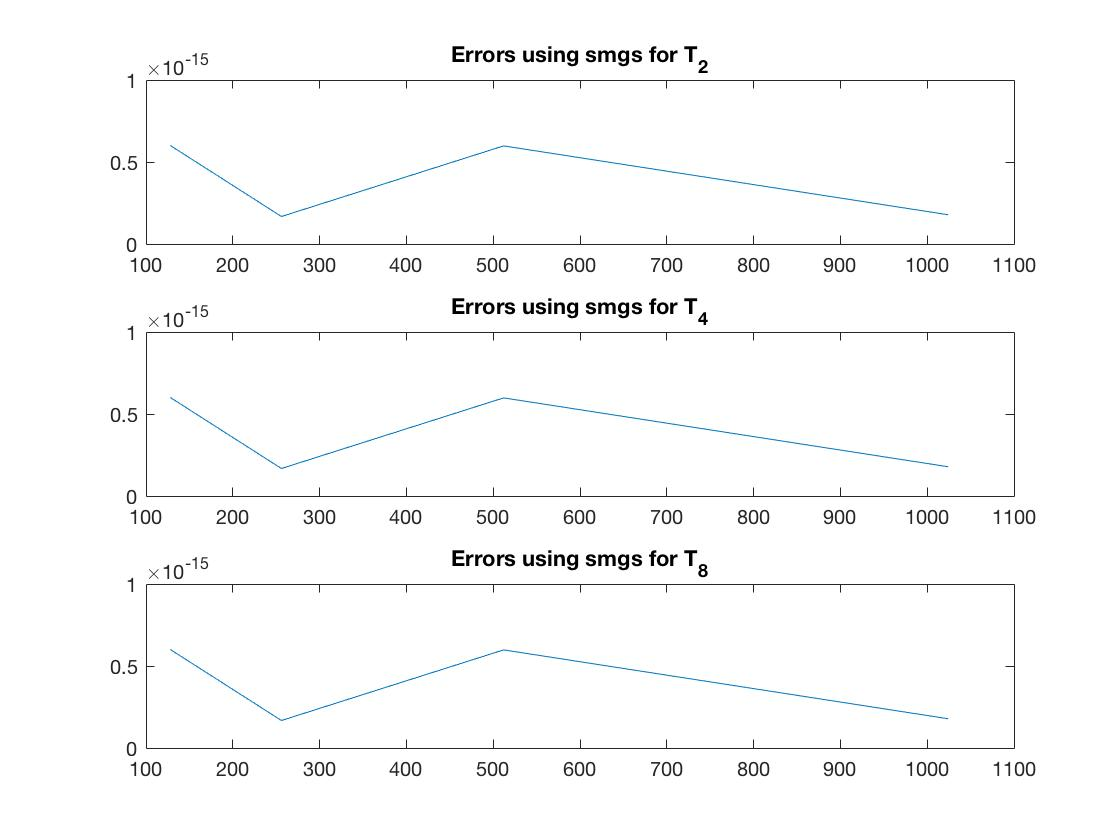
\includegraphics[width=0.49\textwidth]{fig_e_smgs.jpg}
\end{center}

For mmgs, the error decreases as m increases. For smgs, there is no evident increase or decrease in the error as m increases. I believe this is because the error is already so small that it in on the order of machine epsilon and hence increasing the number of points does not make it converge any further.

The differences seen in the methods can be attributed to the fact that in the second method the x points are concentrated near 1 and -1. This allows the projections in the algorithm to effectively capture the increasingly oscillatory behaviour near 1 and -1 which further allows for orthogonal vectors to be formed with greater accuracy leading to smaller errors being compounded in the algorithm as n increases and projections are continuously subtracted.  

%%%%%%%%%%%%%%%%%%%%%%%%%%%%%%%%%%%%%%%%%%%%%%%%%%%%%%%%%%%%
%%%%%%%%%%%%%%%%%%%%%%%%%%%%%%%%%%%%%%%%%%%%%%%%%%%%%%%%%%%%
\newpage
\section{Appendix}

\subsection{Code}
%%%%%%%%%%%%%%%%%%%%%%%%%%%%%%%%%%%%%%%%%%%%%%%%%%%%%%%%%%%%
\subsubsection{Chebyshev\_mmgs.m}

This file contains the function that computes N chebyshev polynomials given equally spaced x points using the modified modified Gram-Schmidt algorithm.

\begin{lstlisting}
function [V] = chebyshev_mmgs(x, n)
% Computes N chebyshev polynomials over m equally spaced x points

[m, ~] = size(x);
% Construct the resulting Vandermonde matrix
V = zeros(m,n); 
for i = 1:n
    V(:,i) = x.^(i-1);
end
% Compute the first n Chebyshev polynomials and store them in V
R = zeros(m,n); % Initialize R
w = (1 - x.^2).^(-1/2); % Compute the values of the weight function
for i = 1:n
    R(i,i) = ( V(:,i)' * ( V(:,i) .* w)) ^ (1/2); % modified norm 
    % It is worth noting that I do not multiply by delta_x in the norm as we later normalize the polynomials.
    q = V(:,i)/R(i,i);
    for j = i+1:n
        R(i,j) = q' * ( V(:,j) .* w); % modified norm
        V(:,j) = V(:,j) - R(i,j) * q;
    end
    V(:,i) = q;
end
%Find the values of the polynomials at the last x value
T = zeros(n,1); 
T(1) = 1;
T(2) = x(m);
for i = 3:n
    T(i) = 2 * x(m) * T(i-1) - T(i-2);
end
% Normalize the values of Q
for i = 1:n
    scaling_factor = T(i)/V(m,i);
    V(:,i) = V(:,i) * scaling_factor;
end
\end{lstlisting}
%%%%%%%%%%%%%%%%%%%%%%%%%%%%%%%%%%%%%%%%%%%%%%%%%%%%%%%%%%%%
\subsubsection{a.m}

Produces a plot of the n polynomials over m equally spaced points computed using the function chebyshev\_mmgs().

\begin{lstlisting}
% Yadu Bhageria
% CID: 00733164

m = 128; % Number of x points
n = 8; % Number of polynomials to be computed

% Construct equally spaced points x_i
delta_x = 2/m;
x = zeros(m,1);
for i = 1:m
    x(i) = delta_x / 2 + (i - 1) * delta_x - 1;
end

Q = chebyshev_mmgs(x, n);

% Plot results
clf;
hold on;
for i = 1:n
    plot( x, Q(:,i))
end
xlabel('x');
title(['Yadu Bhageria: Project 0 part a. n = ' num2str(n) ', m = ' num2str(m)]);
hold off;
\end{lstlisting}

%%%%%%%%%%%%%%%%%%%%%%%%%%%%%%%%%%%%%%%%%%%%%%%%%%%%%%%%%%%%
\subsubsection{Chebyshev\_smgs.m}

This file contains the function that computes N chebyshev polynomials given equally spaced $\theta$ points for x = cos($\theta$) using the standard modified Gram-Schmidt algorithm.

\begin{lstlisting}
function [V] = chebyshev_smgs(x, n)
% Computes N chebyshev polynomials over m equally spaced xtheta points for
% x = cos(theta) with theta over 0 and Pi

[m, ~] = size(x);
% Construct the resulting Vandermonde matrix
V = zeros(m,n); 
for i = 1:n
    V(:,i) = x.^(i-1);
end
% Compute the first n Chebyshev polynomials and store them in V
R = zeros(m,n); % Initialize R
w = (1 - x.^2).^(-1/2); % Compute the values of the weight function
for i = 1:n
    R(i,i) = norm(V(:,i)); % standard norm
    % Similarly it is worth noting that I do not multiply by delta_theta in this norm as we later normalize the polynomials.
    q = V(:,i)/R(i,i);
    for j = i+1:n
        R(i,j) = q' * V(:,j); % standard norm
        V(:,j) = V(:,j) - R(i,j) * q;
    end
    V(:,i) = q;
end
%Find the values of the polynomials at the last x value
T = zeros(n,1); 
T(1) = 1;
T(2) = x(m);
for i = 3:n
    T(i) = 2 * x(m) * T(i-1) - T(i-2);
end
% Normalize the values of Q
for i = 1:n
    scaling_factor = T(i)/V(m,i);
    V(:,i) = V(:,i) * scaling_factor;
end
\end{lstlisting}
%%%%%%%%%%%%%%%%%%%%%%%%%%%%%%%%%%%%%%%%%%%%%%%%%%%%%%%%%%%%
\subsubsection{b.m}

Produces a plot of the n polynomials over m points, spaced evenly for $\theta$ when x = $cos(\theta)$, computed using the function chebyshev\_smgs().

\begin{lstlisting}
% Yadu Bhageria
% CID: 00733164

% Consider the substitution x = cos(theta)

m = 128; % Number of x points
n = 8; % Number of polynomials to be computed

% Construct equally spaced points over theta for x = cos(theta)
x = zeros(m,1);
for i = 1:m
    x(i) = cos( pi * ( 2 * i - 1) / ( 2 * m));
end

Q = chebyshev_smgs(x, n);

% Plot results
clf;
hold on;
for i = 1:n
    plot( x, Q(:,i))
end
xlabel('x');
title(['Yadu Bhageria: Project 0 part b. n = ' num2str(n) ', m = ' num2str(m)]);
hold off;
\end{lstlisting}


%%%%%%%%%%%%%%%%%%%%%%%%%%%%%%%%%%%%%%%%%%%%%%%%%%%%%%%%%%%%
\subsubsection{c.m}

Computes the errors for the modified modified Gram-Schmidt (mmgs) algorithm and the standard modified Gram-Schmidt algorithm (smgs) over values of m = 128, 256, 512, and 1024.

\begin{lstlisting}
% Yadu Bhageria
% CID: 00733164

m_vals = [128, 256, 512, 1024]; % Number of points
n = 9; % Number of polynmials to be computed

E_mmgs = zeros(3,4); % To store the error values for each polynomial with mmgs
E_smgs = zeros(3,4); % To store the error values for each polynomial with smgs

for index = 1:4
    m = m_vals(index);
    
    % Construct equally spaced points x_i
    delta_x = 2/m;
    x = zeros(m,1);
    for i = 1:m
        x(i) = delta_x / 2 + (i - 1) * delta_x - 1;
    end
    
    w = (1 - x.^2).^(-1/2); % Compute weight values for the error
    % Compute the exact values of the chebyshev polynomoials for current x
    T_m = zeros(m,n);
    T_m(:,1) = 1;
    T_m(:,2) = x;
    for i = 3:9
        T_m(:,i) = 2 * x .* T_m(:,i-1) - T_m(:,i-2);
    end
    
    Q_m = chebyshev_mmgs(x, n); % Compute the chebyshev polynomials using the modified MGS method
    
    % Construct equally spaced points over theta for x = cos(theta)
    for i = 1:m
        x(i) = cos( pi * ( 2 * i - 1) / ( 2 * m));
    end
    
    Q_s = chebyshev_smgs(x, n); % Compute the chebyshev polynomials using the standard MGS method
    
    % Compute the exact values of the chebyshev polynomoials for current x
    delta_theta = pi/m;
    T_s = zeros(m,n);
    T_s(:,1) = 1;
    T_s(:,2) = x;
    for i = 3:9
        T_s(:,i) = 2 * x .* T_s(:,i-1) - T_s(:,i-2);
    end
    
    poly_num = 2;
    for i = 1:3
        E_mmgs(i,index) = sqrt(delta_x * sum( ( T_m(:,poly_num + 1) - Q_m(:,poly_num + 1) ).^2 .* w));
        E_smgs(i,index) = sqrt(delta_theta *  sum(( T_s(:,poly_num + 1) - Q_s(:,poly_num + 1) ).^2));
        poly_num = poly_num*2;
    end
end

Table_mmgs = table(E_mmgs(:,1),E_mmgs(:,2),E_mmgs(:,3),E_mmgs(:,4), 'VariableNames',{'M128' 'M256' 'M512' 'M1024'}, 'RowNames',{'T_2' 'T_4' 'T_8'})
Table_smgs = table(E_smgs(:,1),E_smgs(:,2),E_smgs(:,3),E_smgs(:,4), 'VariableNames',{'M128' 'M256' 'M512' 'M1024'}, 'RowNames',{'T_2' 'T_4' 'T_8'})

% Plot results
clf;
figure;
for i = 1:3
    subplot(3,1,i);
    plot( m_vals, E_mmgs(1,:));
    title(['Errors using mmgs for T_' num2str(2^i)]);
end

figure;
for i = 1:3
    subplot(3,1,i);
    plot( m_vals, E_smgs(1,:));
    title(['Errors using smgs for T_' num2str(2^i)]);
end
\end{lstlisting}

\end{document}
